% Autor: Simon May
% Datum: 2017-10-05
% Diese Datei bietet ein minimalistisches Grundgerüst für ein LaTeX-Dokument,
% z.B. für die Bearbeitung der Aufgaben.
\documentclass[
	% Papierformat
	a4paper,
	% Schriftgröße (beliebige Größen mit „fontsize=Xpt“)
	12pt,
	% Schreibt die Papiergröße korrekt ins Ausgabedokument
	pagesize,
	% Sprache für z.B. Babel
	ngerman
]{scrartcl}

% Achtung: Die Reihenfolge der Pakete kann (leider) wichtig sein!
% Insbesondere sollten (so wie hier) babel, fontenc und inputenc (in dieser
% Reihenfolge) als Erstes und hyperref und cleveref (Reihenfolge auch hier
% beachten) als Letztes geladen werden!

% Silbentrennung etc.; Sprache wird durch Option bei \documentclass festgelegt
\usepackage{babel}
% Verwendung der Zeichentabelle T1 (Sonderzeichen etc.)
\usepackage[T1]{fontenc}
% Legt die Zeichenkodierung der Eingabedatei fest, z.B. UTF-8
\usepackage[utf8]{inputenc}
% Schriftart
\usepackage{lmodern}
% Zusätzliche Sonderzeichen
\usepackage{textcomp}

% Mathepaket (intlimits: Grenzen über/unter Integralzeichen)
\usepackage[intlimits]{amsmath}
% Ermöglicht die Nutzung von \SI{Zahl}{Einheit} u.a.
\usepackage{siunitx}
% Zum flexiblen Einbinden von Grafiken (\includegraphics)
\usepackage{graphicx}
% Abbildungen im Fließtext
\usepackage{wrapfig}
% Abbildungen nebeneinander (subfigure, subtable)
\usepackage{subcaption}
% Funktionen für Anführungszeichen
\usepackage{csquotes}
% Zitieren, Bibliographie
\usepackage{biblatex}


% Verlinkt Textstellen im PDF-Dokument
\usepackage[unicode]{hyperref}
% "Schlaue" Referenzen (nach hyperref laden!)
\usepackage{cleveref}

% siunitx: Deutsche Ausgabe, Messfehler getrennt mit ± ausgeben
\sisetup{
	locale=DE,
	separate-uncertainty
}

 


\begin{document}
\begin{titlepage}
	\centering
	{\scshape\LARGE Versuchsbericht zu \par}
	\vspace{1cm}
	{\scshape\huge Stickstofflaser, Untersuchung der Eigenschaften eines Lasers am Beispiel des Stickstofflasers     \par}
	\vspace{2.5cm}
	{\LARGE Gruppe 6 Mo\par}
	\vspace{0.5cm}
	{\large Nils Kulawiak (E-Mail: n\_kula01@wwu.de) \par}
	{\large Oliver Brune (E-Mail: o\_brun02@wwu.de) \par}
	{\large Anthony Pietz (E-Mail: a\_piet09@wwu.de) \par}
	\vfill
	durchgeführt am 14.01.2019\par
	
	\vfill
	betreut von Tobias Reiker\par
	
	\vfill
	{\large \today\par}
\end{titlepage}

\tableofcontents
\newpage

\section{Kurzfassung}
In diesem Versuch soll ein Stickstofflaser auf verschiedene Eigenschaften untersucht werden. Dazu wird zuerst Energie der einzelnen Impulse, die Repetitionsrate und die Impulsdauer des Lasers bestimmt.
Bei der Beobachtung des Spektrums könne zwei Peaks erkannt werden. Der erste Peak bei ($337 \pm 3$)nm und der zweite Peak bei etwa $800$nm. Bei genauerer Betrachtung der Werte stellt sich heraus, dass der erste Peak in Sättigung aufgenommen wurde. Weiterhin konnte innerhalb des ersten Peaks eine feinere Aufspaltung beobachtet werden. Dieser Peak kann in einen globalen und einen lokalen Peak gegliedert werden. Der lokale Peak ist bei einer Wellenlänge von etwa $330$ nm zu beobachten.
Die Halbwärtsbreite des globalen Peaks beträgt nach theoretischen Berechnungen $0,0012$nm und nach experimentellen Messungen $5,1 \pm 0,2$.
Als nächstes wurde der Laserstrahl auf eine Farbstoffküvette geleitet. Diese wurde aufgrund der hoch energetischen Strahlung des Lasers angeregt und emittierte ihr eigenes Spektrum, aufgrund dieses Spektrums konnte der Stoff innerhalb der Farbstoffküvette gefüllt werden. Der Stoff konnte zu einer Mischung aus Coumarin 153 und Rhodamine 6G bestimmt werden.



\section{Methode}
Der Stickstofflaser besteht aus zwei gleich geladenen Platten,die über einen Widerstand verbunden sind, und einer Funkenstrecke. Die beiden Platten liegen auf einer leitenden, geerdeten Unterlage, sind jedoch durch eine Folie davon isoliert und funktionieren damit als Elektroden. Zunächst haben die beiden Platten durch Aufladen das gleiche Potential, durch eine Entladung auf die Funkenstrecke entlädt sich eine der beiden Platten schlagartig, was zu einer großen Potentialdifferenz führt. Dadurch kommt es zu einer weiteren Entladung zwischen den beiden Platten an der Stelle, an der sie sich am nächsten sind, wodurch es zu einem Zusammenstoß mit den Stickstoffmolekülen kommt. Deshalb werden die Stickstoffmoleküle angeregt und senden durch hauptsächlich spontane Emission Photonen aus. %bin ich mir nicht ganz sicher nochmal überprüfen pls%

Für die ersten 3 Messungen von Pulsenergie, Repetitionsrate und Impulsdauer des Lasers, sind einfache Messungen mit einer Photodiode, die an einem Oszilloskop angeschlossen ist, nötig.
Bei der Bestimmung der Pulsenergie wird ein einzelner Impuls komplett aufgezeichnet und die niedrigste Spannung herausgesucht, um die Energie zu berechnen. 
Für die Repetitionsrate müssen mehrere Impulse aufgenommen wurden, wodurch über den Abstand der einzelnen Impulse die Rate ausgerechnet wird.
Bei der Impulsdauer wurden wiederum ein Impuls aufgenommen und die Dauer dieses Impulses gemessen.

Die ersten beiden Messungen werden, dabei mit einer "langsameren" Diode gemessen, während für die letztere die schnelle Diode zu benutzten ist. Das ist der Fall, weil die schnellere Photodiode zwar schneller auf Änderungen reagiert, allerdings den Nachteil hat, dass sie ebenso schnell übersteuert.

Der untersuchte Stickstofflaser kommt aufgrund seiner Konstruktionsweise ohne Resonator aus, mit dem normalerweise eine bestimmte Wellenlänge und ein festgelegtes Strahlprofil erzeugt werden. Daher wurde im nächsten Versuchsteil die Divergenz des Strahls bestimmt. Hierzu wurde die Intensität des Strahls an verschiedenen Stellen vertikal entlang des Strahldurchmessers im Abstand von $\SI{30}{cm}$ und $\SI{3}{m}$ zum Laser mit einer Photodiode gemessen. Hierfür wurde im Abstand von $\SI{30}{cm}$ alle $\SI{0,5}{mm}$ ein Messwert genommen, im Abstand von $\SI{3}{m}$ wurde jeden Millimeter ein Messwert genommen. Um Messung in diesem feinen Abständen zu realisieren, wurde die Photodiode auf einem Verschiebetisch positioniert, der senkrecht zum Strahl mithilfe einer Mikrometerschraube verstellt wurde.
Anschließend wurde eine Linse in den Strahlgang gestellt, um den Laserstrahl zu kollimieren. Nun wurde die Messung im Abstand von $\SI{3}{m}$ wiederholt, diesmal wurde alle $\SI{0,5}{mm}$ ein Messwert genommen. Da die Leistung des Laserstrahls stark schwankte, wurde für alle Messungen zur Divergenz am Oszilloskop mithilfe der Funktion "Aquire" der Mittelwert der Spannung aus 64 Werten gebildet.

\begin{figure}[h!]
	\centering
	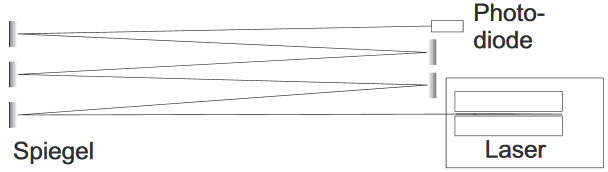
\includegraphics[scale=0.9]{skizze_c.png}
	\caption{Schematische Darstellung des Aufbaus der Messreihe zur Lichtgeschwindigkeit}
	\label{skizze_c}
\end{figure}

Im nächsten Abschnitt sollte mithilfe des Laserstrahls die Lichtgeschwindigkeit bestimmt werden. Dazu wird zuerst der Strahl mithilfe eines Strahlteilers im Abstand von $\SI{13,5}{cm}$ zum Laser teilweise um $90$° abgelenkt. Im um $90$° reflektierten Strahl wurde eine Photodiode im Abstand von $\SI{8,3}{cm}$ platziert. Diese wird mit dem Oszilloskop verbunden. Auch in den nicht reflektierten Strahl wird im Abstand von $\SI{8,3}{cm}$ eine Photodiode platziert. Diese wird auch mit Oszilloskop verbunden, allerdings mit einem deutlich längeren Kabel. Da das Signal im längeren Kabel einen längeren Weg zurücklegen muss als das Signal im kürzeren Kabel, erreichen die Signale das Oszilloskop zu unterschiedlichen Zeiten.
Anschließend wird die zweite Photodiode um drei Meter vom Laser entfernt und der Strahl, wie bereits im vorherigen Versuchsteil, mit einer Sammellinse, die in einem Abstand von $\SI{55,5}{cm}$ zum Laser positioniert wird, kollimiert. Unter diesen veränderten Parametern wird die Messung wiederholt. Die Entfernung, die das Licht zur zweiten Photodiode zurücklegen muss, wird nun in Schritten von drei Metern immer weiter erhöht. Hierzu werden, wie in \cref{skizze_c} dargestellt, Spiegel verwendet, die den Laserstrahl über immer größere Strecken zur Photodiode lenken.
Aus der Zeitdifferenz zwischen den beiden Signalen und der Distanz zwischen den optischen Instrumenten lässt sich nun die Lichtgeschwindigkeit bestimmen.
Auch bei dieser Messreihe wurde aufgrund der stark schwankenden Leistung des Lasers am Oszilloskop mithilfe der Funktion "Aquire" der Mittelwert aus $64$ Messungen verwendet.

\section{Ergebnis}
Zuerst wird versucht die Pulsenergie des Lasers zu bestimmen. Dazu muss zuerst die niedrigste Spannung ermittelt werden. Um das herauszufinden, wird der niedrigste Weert aus \cref{Energie} genommen. 

\begin{figure}[h!]
	\centering
	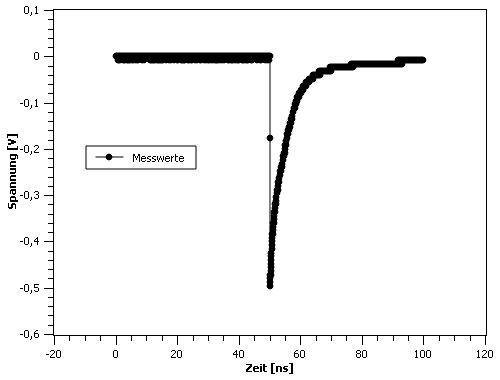
\includegraphics[scale=0.7]{Energie.png}
	\caption{Puls zur Berechnung der Energie}
	\label{Energie}
\end{figure}

Über die Formel
\begin{equation}
E_{p} = \dfrac{1 \mu J}{50mV}U_{min} = \SI{9,92 \pm 0,30}{\mu J} 
\label{eq:Energie}
\end{equation}
lässt sich dann die Energie des Pulses bestimmen.

Die Unsicherheit für die Messung der Spannung liegt bei Einzelmessungen bei 3\%. Daraus folgt die Unsicherheit in \cref{eq:Energie}

Daraufhin soll die Repetitionsrate des Lasers bestimmt werden. Dazu wurden mehrere Pulse in \cref{Rep} aufgenommen und jeweils der Abstand zwischen ihnen bestimmt. Dazu wird jeweils der größte Zeitpunkt gewählt an dem der Puls noch messbar ist und dann die Differenz gebildet. Aus dem Mittelwert ergibt sich eine Repetitionsrate von $t_{Rep}$ = $\SI{0,0814 \pm 0,0006}{s]}$, was einer Frequenz von f = $\SI{12,29 \pm 0,09}{Hz}$ entspricht. Das stimmt auch mit dem vom Oszilloskop abgelesenen Wert von f = $\SI{12,15}{Hz}$ überein.

\begin{figure}[h!]
	\centering
	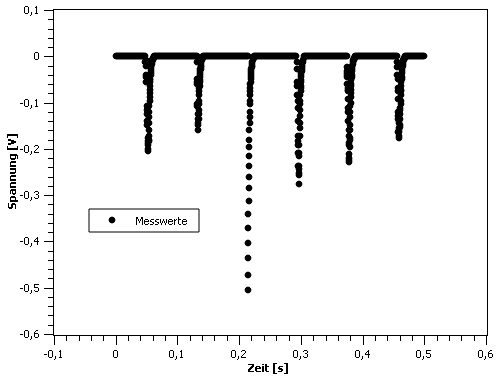
\includegraphics[scale=0.7]{Rep.png}
	\caption{Mehrere Pulse zur Bestimmung der Repetitionsrate}
	\label{Rep}
\end{figure}

Die Unsicherheit von einem Zeitintervall für Einzelmessungen beträgt 
\begin{equation}
u(\Delta t)[\text{s}] = \text{Abtastintervall} + \text{Ablesung} *10^{-4} +0,6*10^{-9}.
\label{eq:ut}
\end{equation}
Aus der Bildung des Mittelwerts folgt die Unsicherheit von $t_{Rep}$.


Als nächstes soll die Impulsdauer eines einzelnen Impulses bestimmt werden. Dies wird mithilfe von \cref{Pulsdauer} versucht. Dort ist auch sichtbar, dass die Pulse näherungsweise einer Gaußkurve haben. Die Halbwertsdauer lässt sich relativ einfach bestimmen. Dazu wird einfach geschaut, ab wann die Spannung auf die Hälfte des Maximalwertes abfällt. Daraus ergibt sich eine Halbwertsdauer von $t_{\tfrac{1}{2}} = \SI{13,3 \pm 0,6}{ns}$. Schwieriger ist es die Gesamtdauer des Pulses zu bestimmen, da die Spannung für kleine Werte anfängt zu schwanken. Wenn die Gesamtdauer so definiert ist, dass der Puls zu Ende ist, sobald die Spannung unter 0,24V fällt, dann ergibt sich eine Dauer des Gesamtimpulses von $t = \SI{14,180 \pm 0,0014}{ns}$. Die Definition wurde so gewählt, da ab diesem Wert die Spannung anfangen hat stark zu schwanken, allerdings ist diese Definition relativ willkürlich gewählt. 

Die Unsicherheit wurde dabei analog mit \cref{eq:ut} berechnet.

\begin{figure}[h!]
	\centering
	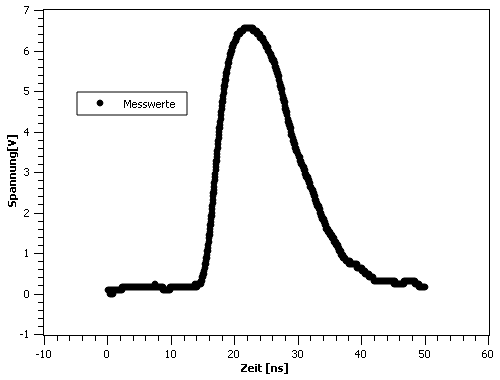
\includegraphics[scale=0.7]{Pulsdauer.png}
	\caption{Genau Auflösung eines Pulses zur Bestimmung der Pulsdauer}
	\label{Pulsdauer}
\end{figure}

\subsection{Divergenz}
Die Intensitätsverteilung des Laserstrahls in unterschiedlichen Abständen vom Laser ist in \cref{breite} dargestellt.

\begin{figure}[h!]
	\centering
	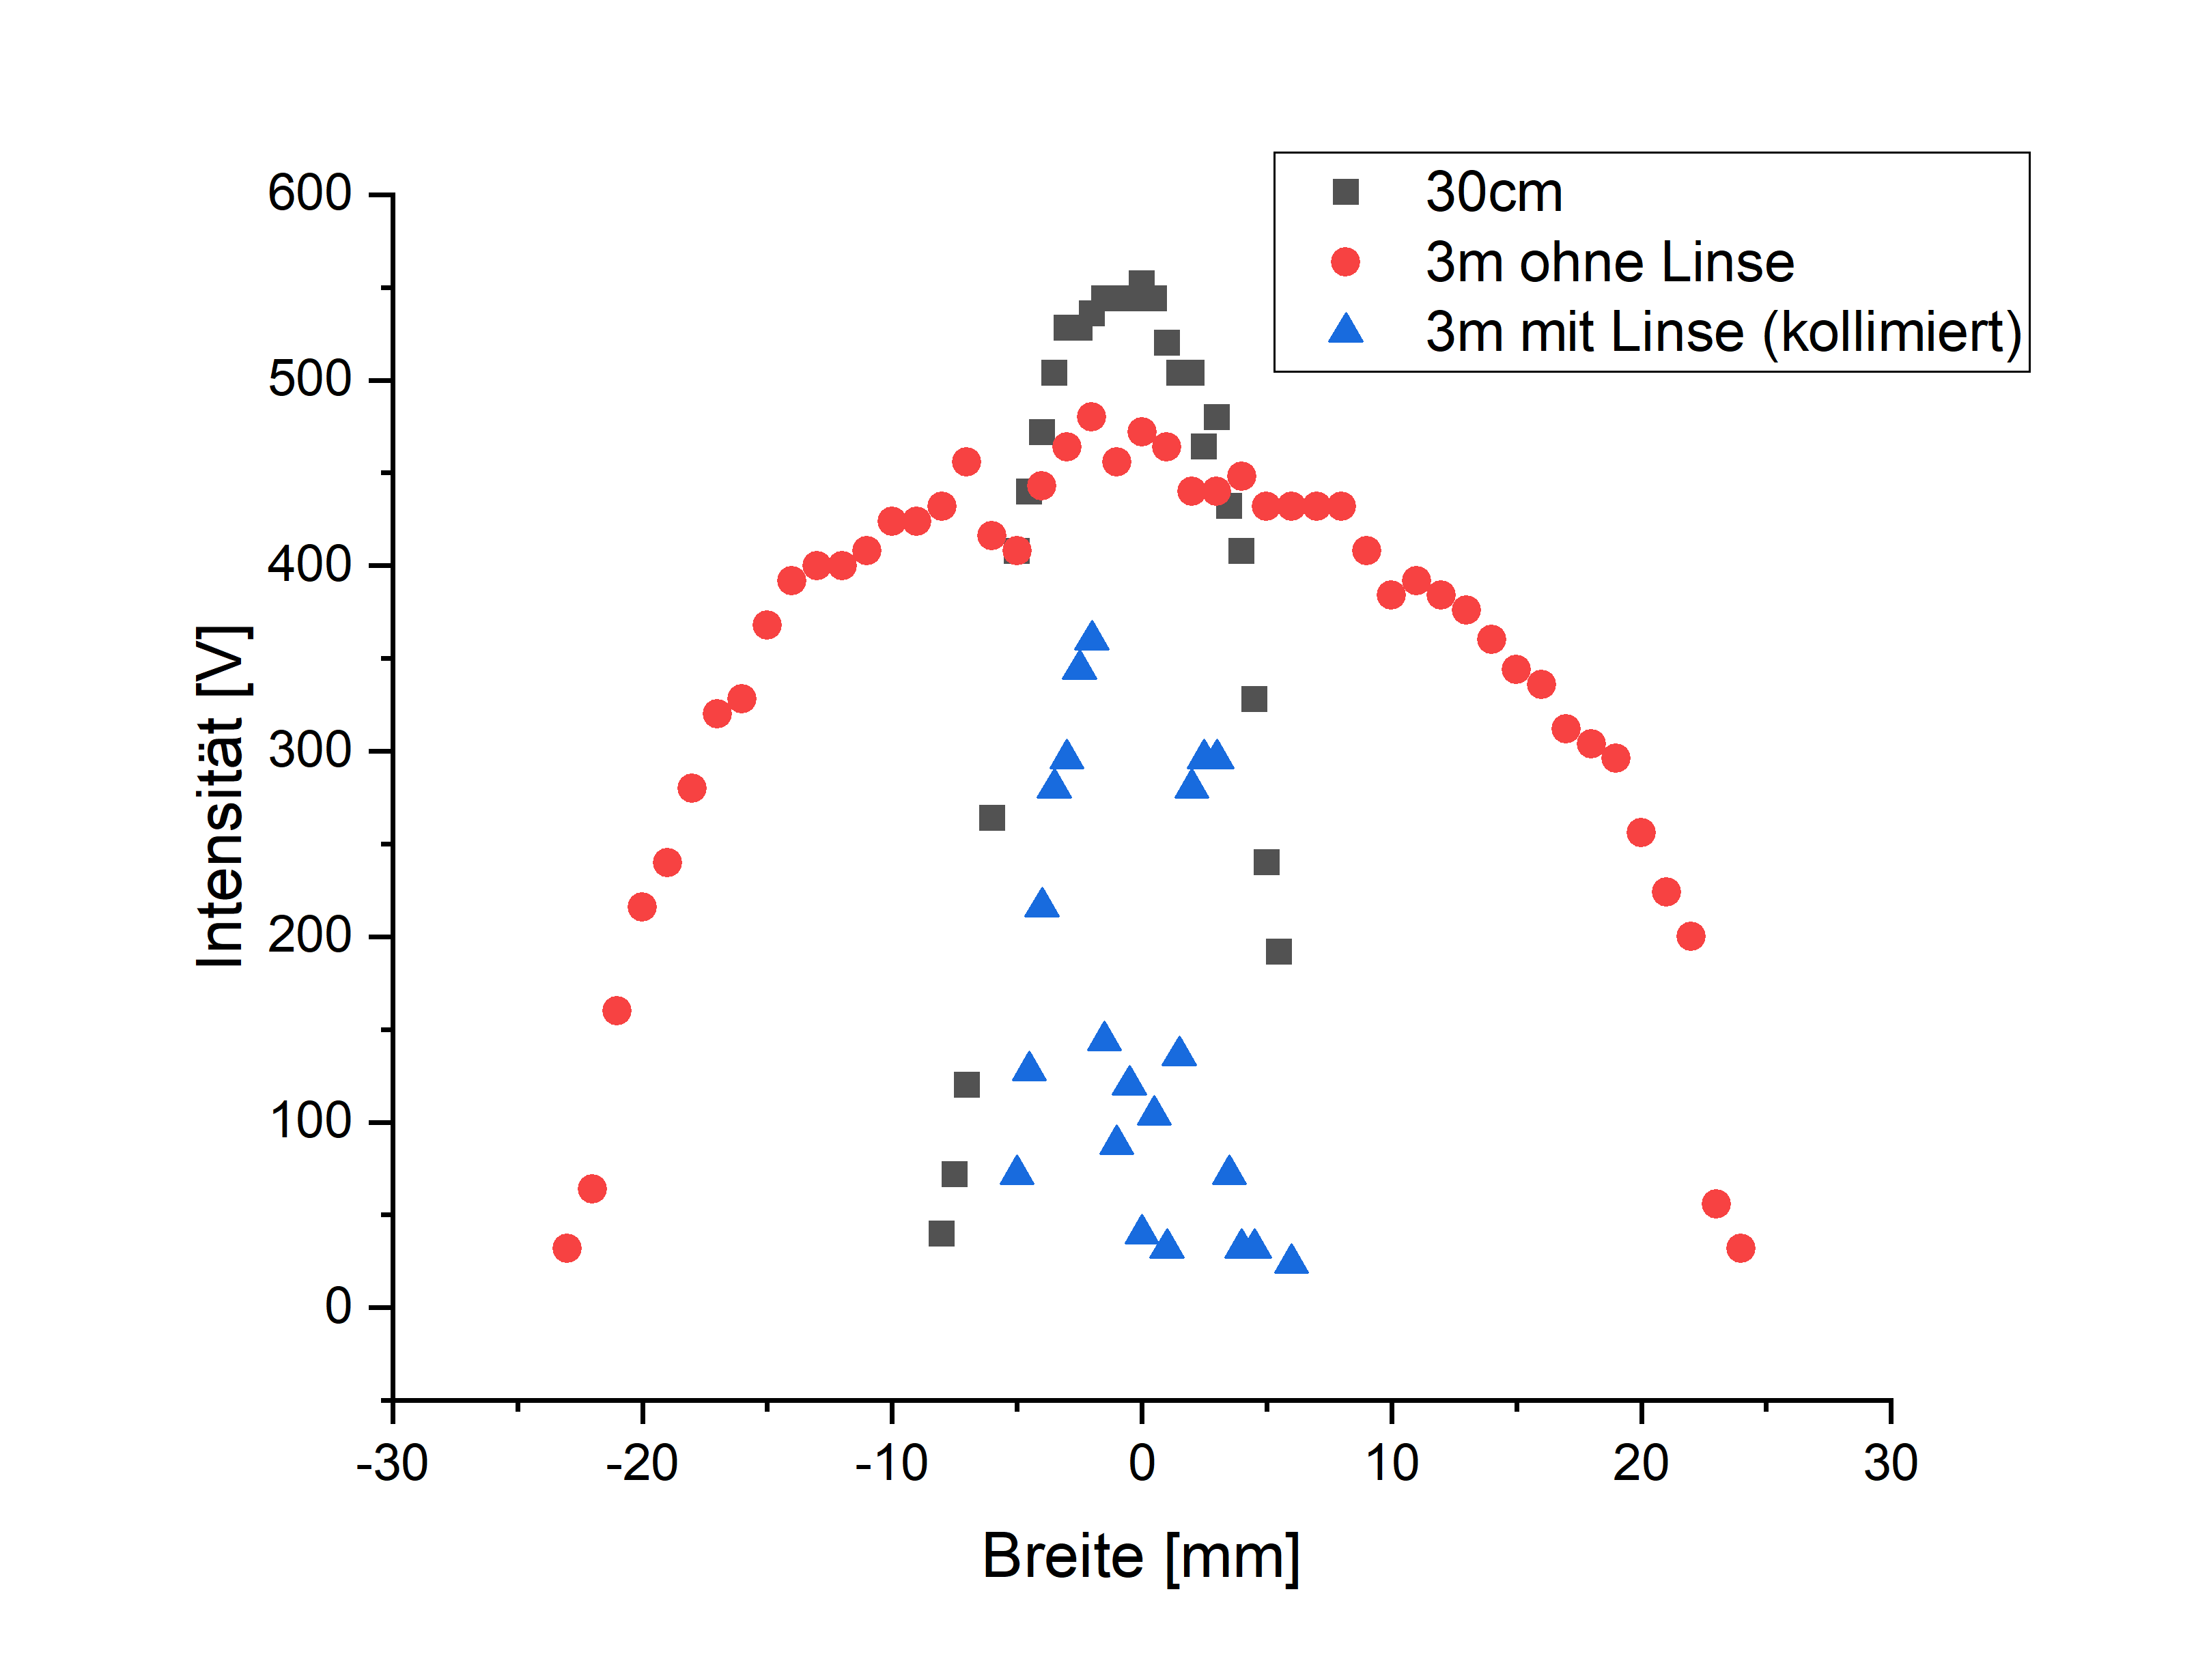
\includegraphics[scale=0.5]{breite.png}
	\caption{Intensität des Laserstrahls aufgetragen gegen den waagerechten Abstand vom Maximum der Intensität in 30cm und 3m Entfernung, einmal mit und einmal ohne Linse im Strahlgang}
	\label{breite}
\end{figure}

Die Messung im Abstand von 30cm ergibt eine schmale, hohe Gaußkurve, da der Laserstrahl an diesem Punkt noch einen kleinen Durchmesser besitzt. In $\SI{3}{m}$ Entfernung ist der Strahl bereits deutlich breiter, außerdem liegt das Intensitätsmaximum etwa $\SI{80}{V}$ niedriger als in $\SI{30}{cm}$ Entfernung. Diese beiden Kurven entsprechen den intuitiven Erwartungen. Die Verbreiterung des Strahls ist auch in \cref{strahlprofil} deutlich sichtbar, wo das Strahlprofil des Lasers linear genähert wurde. Als Rand des Lasers wurden hier die Orte definiert, an denen die Intensität auf die Hälfte des Maximums abgefallen war. Der Strahl verbreitert sich offenbar ohne die Verwendung optischer Instrumente um $\SI{1,056\pm0,025}{mm}$ pro Zentimeter Abstand zum Laser.

\begin{figure}[h!]
	\centering
	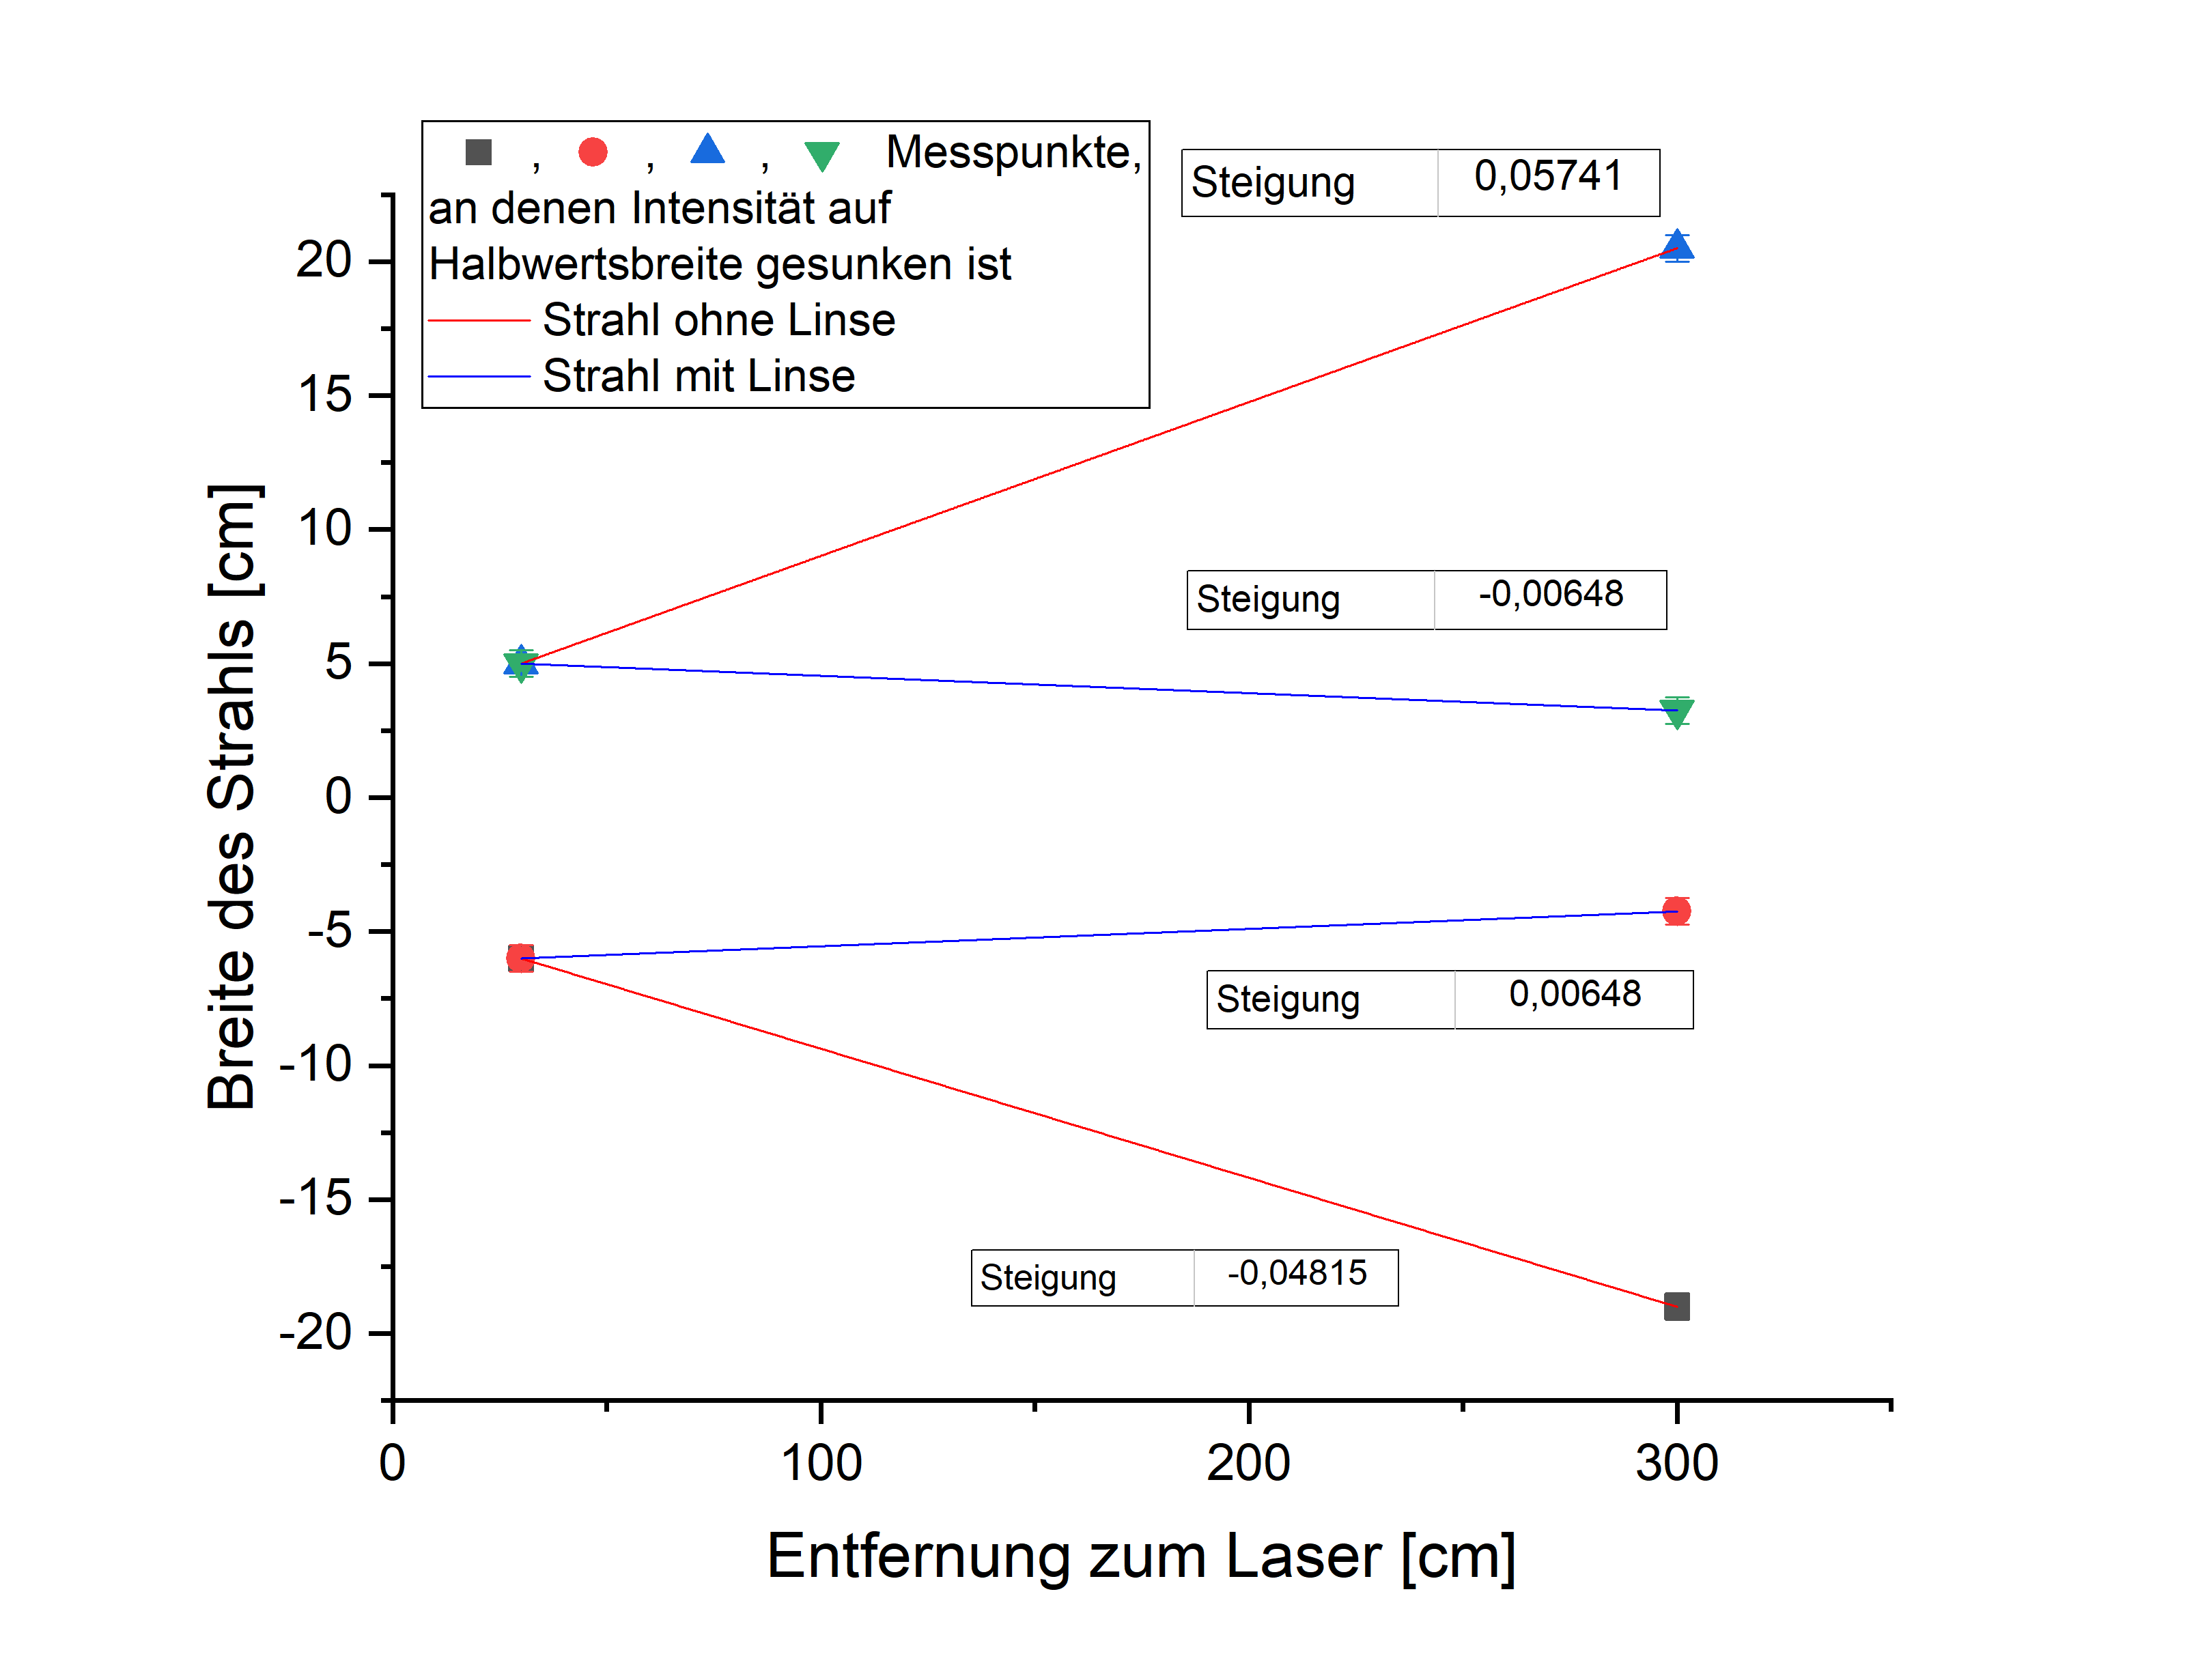
\includegraphics[scale=0.5]{strahlprofil.png}
	\caption{Strahlprofil des unveränderten und des kollimierten Strahls.}
	\label{strahlprofil}
\end{figure}

Um diesen Effekt, der die Strahlqualität deutlich reduziert, zu verhindern, wird nun zur Kollimierung des Strahls in einem Abstand von $\SI{55,5}{cm}$ eine Sammellinse positioniert. Mit dieser Linse im Strahlgang wurde die dritte Messreihe aufgenommen. An den Rändern verhält sich der Laser ähnlich wie in den vorherigen Messreihen, die Intensität steigt zuerst stark an. In der Mitte des Strahls allerdings, wo das Intensitätsmaximum erwartet wird, fällt die Intensität stark ab, sodass der Laserstrahl fast komplett verschwindet. Dieses Verhalten war so nicht erwartet worden, die Intensitätsverteilung weicht stark von der charakteristischen Intensitätsverteilung eines Lasers, wie sie in den beiden vorherigen Messreihen beobachtet werden konnte, ab. Vielmehr ähnelt sie zwei parallel nebeneinander verlaufenden Laserstrahlen.

In \cref{strahlprofil} wurden zur Ermittlung des Strahlprofils die äußeren Halbwertsbreiten zu den beiden Maxima als Breite des gesamten Strahls verwendet. Hieraus ergab sich, dass sich der Strahl hier nicht verbreitert, sondern sogar um $\SI{0,130\pm0,025}{mm}$ pro Zentimeter Abstand vom Laser schmaler wird. Die Linse wurde also nicht optimal positioniert, da sie den Strahl zu stark fokussiert.

Ein möglicher Grund für die untypische Strahlcharakteristik der letzten Messreihe ist, dass die Sammellinse nicht optimal positioniert wurde. Da sie den Strahl nicht nur kollimiert, sondern sogar schmaler werden lässt, wäre es möglich, das die äußeren Anteile des Strahls, die in die Mitte gebrochen werden, mit den Anteilen im Zentrum des Strahls destruktiv interferieren, sodass keine Intensität gemessen wurde. Außerdem lieferte der Laser zu diesem Zeitpunkt des Versuch nur eine sehr stark schwankende Leistung, was die Messwerte weiter verfälscht haben könnte.

Die Unsicherheit bei der Messung der Breite beträgt nur $\SI{\pm0,005}{mm}$, da sich die Position mit der Mikrometerschraube präzise bestimmen ließ, und spielt daher in der Berechnung keine Rolle. Eine etwas größere Rolle spielt die Unsicherheit beim Ablesen der Halbwertsbreite. Da nur alle $\SI{0,5}{mm}$ bzw. alle $\SI{1}{mm}$ ein Messwert genommen wurde, kann die Unsicherheit der Position der Halbwertsbreite auf $\SI{\pm0,5}{mm}$ abgeschätzt werden. Mithilfe der Fehlerfortpflanzung kann so die Unsicherheit der Verbreiterung des Strahls bestimmt werden. Diese beträgt $\SI{\pm0,025}{mm}$.

\subsection{Lichtgeschwindigkeit}
Die Laserpulse haben, wie in \cref{Pulsdauer} zu erkennen ist, die Form einer Gaußkurve. Um nun die Zeitdifferenz zwischen beiden Signalen zu bestimmen, wird jeweils der früheste Zeitpunkt gewählt, an dem das Signal sichtbar wird. In \cref{lichtgeschwindigkeit} ist gegen diese Zeitdifferenz der Laufzeitunterschied zwischen dem um $90$° abgelenkten Laserstrahl und dem nicht abgelenkten Laserstrahl aufgetragen. Durch diese Messpunkte wird eine lineare Fitgerade gelegt. Die Steigung dieser Geraden entspricht der Geschwindigkeit des Lichts in der Einheit \SI{}{m/ns}. Die Gerade ist entlang der $y$-Achse nach unten verschoben, da in der Messung des Laufzeitunterschieds nicht die unterschiedliche Länge der beiden Kabel berücksichtigt wurde. Da diese jedoch in allen Messungen konstant ist, kann sie vernachlässigt werden. Umgerechnet ergibt sich aus diesen Messungen eine Lichtgeschwindigkeit von $\SI{301370\pm3970}{km/s}$. In diesem Bereich liegt auch der tatsächliche Wert von etwa $\SI{299 792}{km/s}$. Dies deutet auf eine korrekt durchgeführte Messung hin und stützt den bekannten Wert der Lichtgeschwindigkeit.

\begin{figure}[ht!]
	\centering
	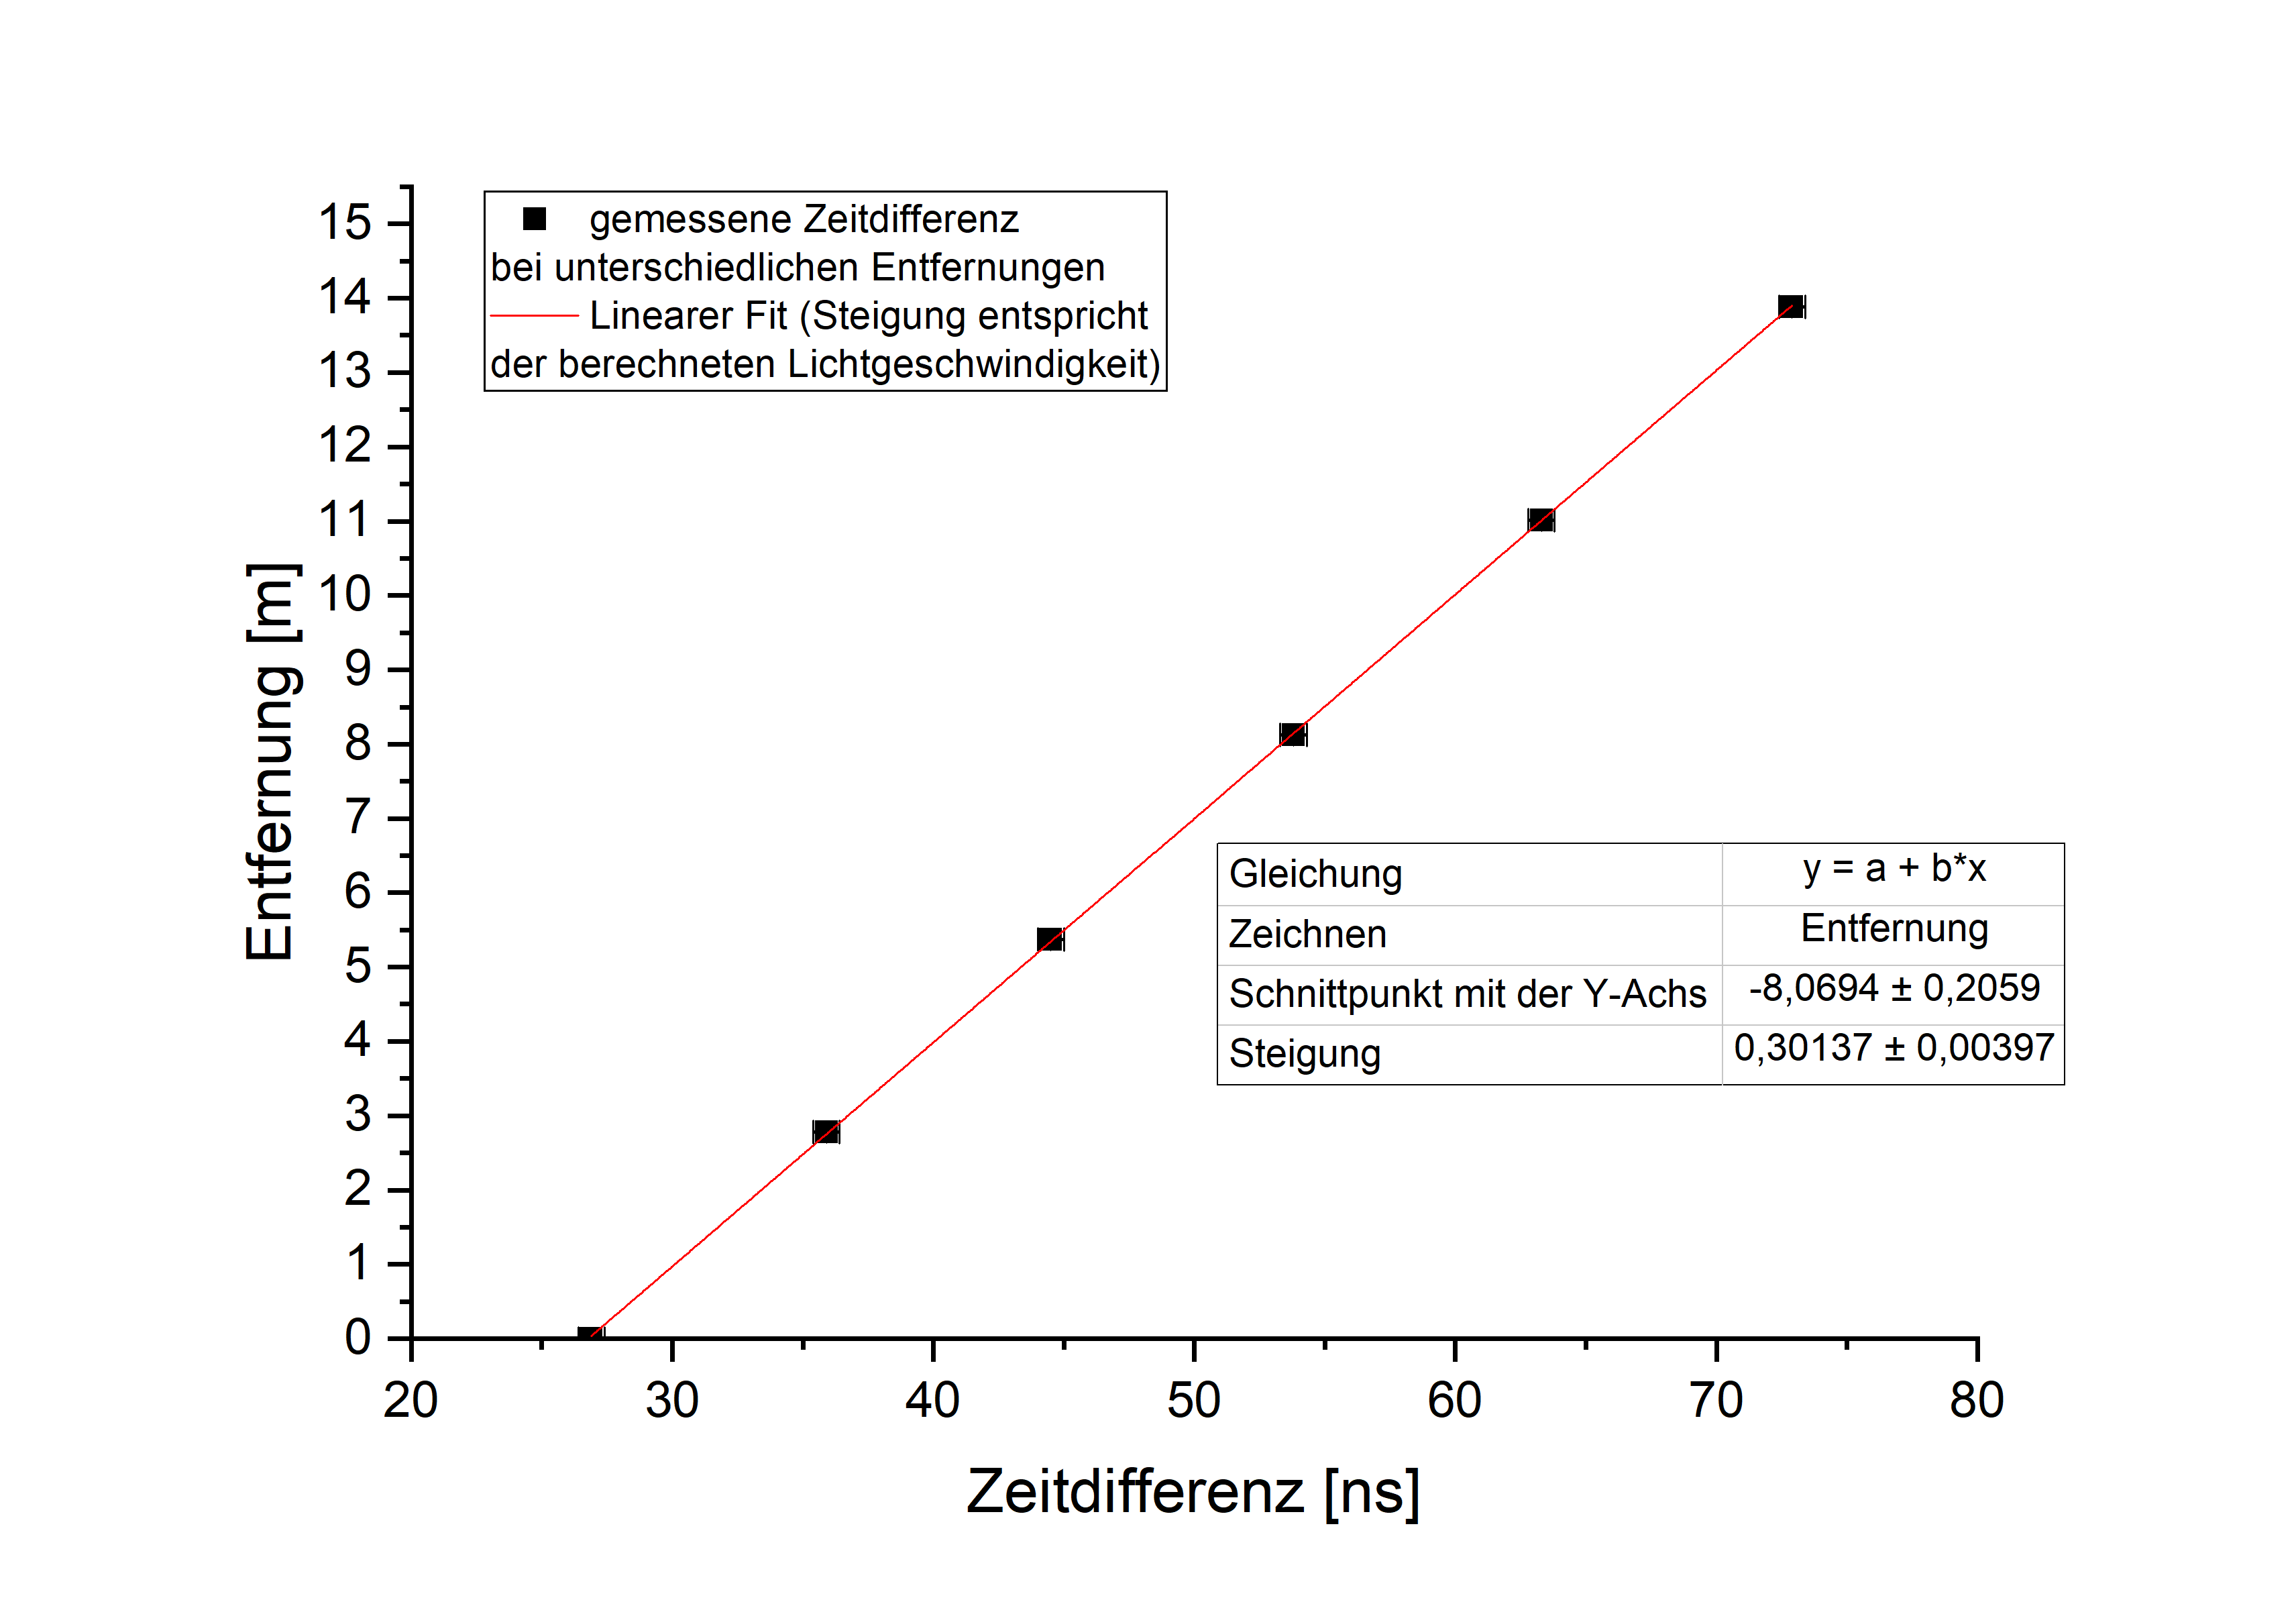
\includegraphics[scale=0.6]{lichtgeschwindigkeit.png}
	\caption{Die Zeitdifferenz zwischen der Detektion der Laserpulse in den beiden Photodioden. Dagegen aufgetragen ist der Laufzeitunterschied des Laserstrahls zwischen den beiden Photodioden.}
	\label{lichtgeschwindigkeit}
\end{figure}

Die Unsicherheit in der Entfernungsmessung, die durch die analoge Messung mit einem Maßband zustande kommt, kann auf $\SI{\pm0,005}{m}$ abgeschätzt werden. Die Unsicherheit der Zeitmessungen bei Verwendung der Funktion "Aquire" ist in der Anleitung des Oszilloskops mit \cref{eq:ut2} angegeben.
\begin{equation}
	u(\Delta t)_\text{Mittelwert} = \pm(\text{Abtastintervall} + \SI{100}{ppm} * \text{Ablesung} + \SI{0,4}{ns})
	\label{eq:ut2}
\end{equation}
Unter Berücksichtigung dieser Unsicherheiten ergibt sich für die Steigung insgesamt eine Unsicherheit von $\SI{\pm0,00397}{m/ns}$.

\subsection{Methoden}
\subsubsection{Übergänge}
In einem Stickstofflaser können verschiedene Übergänge auftreten. Die Elektonen werden vom Grundzustand $X^1\Sigma_u$ in den $C^3\Pi_u$ gehoben und gehen dann in den Metastabilen Zustand $B^3\Pi_g$ über. Diese drei Übergänge stehen, wie folgt in Verbindung zueinander.
\begin{align}
    \lambda_{C^3\Pi_u-B^3\Pi_g} =  \frac{\lambda_{C^3\Pi_u-X^1\Sigma_u}\lambda_{X^1\Sigma_u-B^3\Pi_g}}{\lambda_{C^3\Pi_u-X^1\Sigma_u}-\lambda_{C^3\Pi_u-X^1\Sigma_u}} 
\end{align}

\subsubsection{Linienverbreiterung}
Das Spektrum eines Lasers weißt aufgrund gewisser Effekte eine Verbreiterung einzelner Peaks auf. Hier werden drei Faktoren berechnet. Die drei Effekte sind die natürliche Linienverbreiterung, die Dopplerverbreiterung und die Stoß- und Druckverbreiterung.
Die natürliche Linienverbreiterung ergibt sich quantenmechanisch aus der Energieunbestimmtheit und wird durch 
\begin{align}
    \Delta\nu &= \frac{1}{2\pi\tau}
\end{align}
beschrieben. Dabei stellt $\nu$ die Frequenz und $\tau$ die Lebensdauer dar. In unserem Fall beträgt die Lebensdauer $10$ns.
Daraus errechnete sich ein Wert von 
\begin{align*}
     \Delta\nu &= 1,6 \cdot 10^7 Hz
\end{align*}
Die Dopplerverbreiterung findet statt, da sich die Moleküle mit einer gewissen Geschwindigkeit bewegen. Diese wird durch 
\begin{align}
    \Delta\nu_\text{D} &= 7,16 \cdot 10^{-7} \sqrt{\frac{T}{M}} \nu_0
\end{align}
berechnet. Hierbei stellt T die Raumtemperatur ($300$K)  und M die molare Masse für $\text{N}^2$ dar.
Daraus errechnete sich ein Wert von
\begin{align*}
      \Delta\nu_\text{D} &= 2,95 \cdot 10^9 Hz
\end{align*}
Der letzte Effekt ist die Druckverbreiterung. Diese wurde durch 
\begin{align}
    \Delta\nu_\text{p} &= \frac{\sqrt{\frac{8}{\pi}}pd^2}{\sqrt{mkT}}
\end{align}
berechnet. Wobei p der Druck, d der Teilchendurchmesser und m die Teilchenmasse ist. Daraus errechnete sich ein Wert von
\begin{align*}
       \Delta\nu_\text{p} &= 3 \cdot 10^8
\end{align*}
Die gesamte Linienverbreiterung beträgt die Summe aller Effekte und beträgt.
\begin{align*}
       \Delta\nu + \Delta\nu_\text{D} +  \Delta\nu_\text{p} &= 3,3 \cdot 10^{-9}Hz
\end{align*}
Im Ortsraum entspricht das $0,0012$nm.

\subsection{Auswertung}
\subsubsection{Beschreibung des Spektrums}
In \cref{Spektrumges} sieht man die gesamte Aufnahme des Spektrums. Es ist ein Hauptintensitätsmaximum bei einer Wellenlänge von etwa 337nm festzustellen. Desweiteren kann ein Nebenmaxima bei ca. 800nm begutachtet werden. An der Abbildung ist zu erkennen, das bei 800nm nur ein einzelner Punkt vorliegt, welcher als Maxima interpretiert werden kann. So lässt sich über diesen Peak aussagen, dass er sehr schmal sein muss.
\begin{figure}[h!] 
	\centering
	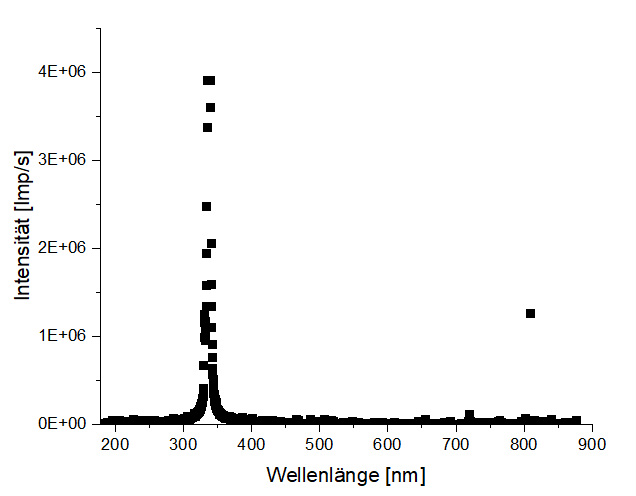
\includegraphics[scale = 1]{gesamt.png}
	\caption{Diese Abbildung zeigt das gesamte Spektrum im sichtbaren Bereich.}
	\label{Spektrumges}
\end{figure}

Anhand dieses Bildes ist zu erkennen,dass es sich bei dem großen Peak im allgemeinen nicht nur um ein Peak gehandelt hat, sondern um zwei. Der Hauptpeak, der bereits in Sättigung verläuft. Dies ist zu erkennen, da bei einer Impulsrate von ca. $4 \cdot 10^6$ Impulsen pro Sekunde eine konstante Zählrate zu beobachten ist. Ebenfalls ist der zweite Peak zu beobachten, dessen Energieniveau nur knapp oberhalb des Energieniveaus des Hauptpeaks liegt.
\begin{figure}[h!]
	\centering
	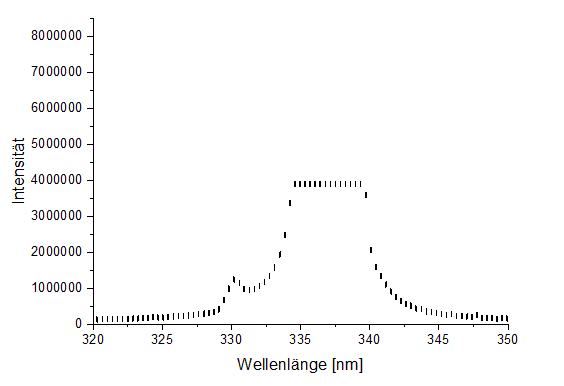
\includegraphics[scale = 1.5]{fitbilfuns.png}
	\caption{Dies ist ein Ausschnitt von \cref{gesamt.png} im Bereich von 320nm bis 350 nm.}
	\label{naherpeak}
\end{figure}

\subsubsection{Übergänge}
In diesem Teil wird das Spektrum des Stickstofflasers untersucht. Dabei treten, die in dem Methodenteil genannten Übergänge auf. Anhand von \cref{naherpeak} ist zu erkennen, dass der Übergang von $X^1\Sigma_u$ in den $B^3\Pi_g$ den Peak darstellen muss, welcher bei $337 \pm 3$nm sein Maximum besitzt. Der Übergang von 
$X^1\Sigma_u$ in den $C^3\Pi_u$-Zustand kann dem kleinen Peak bei etwa $330 \pm 0,1$nm beobachtet werden. Der letzte Peak der im Spektrum zu sehen ist müsste somit den Übergang von $C^3\Pi_u$ in den $B^3\Pi_g$ darstellen. Dieser muss genau die Energie besitzen der Differenz der anderen Peaks, deshalb liegt der im nahen Infrarotbereich, da hier die Übergänge Nah aneinander liegen. Nach dem Methodenteil folgt jedoch, dass der Peak bei $800$nm nicht aus den anderen Beiden Übergängen folgen kann, sodass wir hier den Ursprung des Peaks nicht kennen. 

\subsubsection{Bandbreite}
Um die Bandbreite des Peaks zu bestimmen wurde die Graphik \cref{naherpeak} herangezogen. Für die Bandbreite interessiert nur der Hauptpeak, da der kleine Peak nur kaum zu der Gesamtfläche beiträgt. Anhand der Modellierung des Hauptpeaks kann dann der kleinere Peak unbeachtet gelassen werden. Ebenfalls die Sättigungsgrenze des Hauptpeak ist für eine geeignete Modellierung nicht erwünscht. Wenn ein Peak in Sättigung aufgenommen wird, ist es logisch, dass wenn die Sättigung als Maximum betrachtet wird, die Halbwärtsbreite stark anwächst. Somit ist anhand der Messwerte aufjedenfall eine obere Grenze für die Halbwärtsbreite gegeben.
Somit entsteht \cref{bilfun}. 
\begin{figure}[h!]
	\centering
	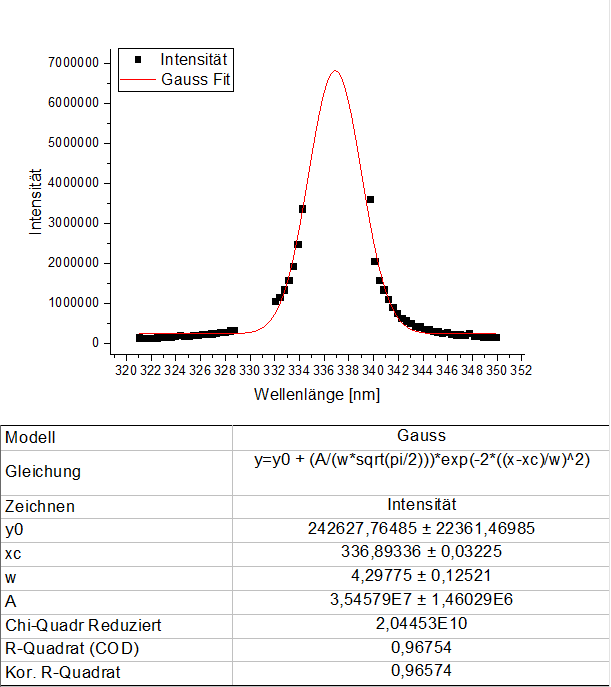
\includegraphics[scale = 1]{fitsnip.png}
	\caption{Die Messpunkte sind die Manipulierten Punkte aus \cref{naherpeak}. Die rote Kurve ist die mit OriginPro gefittete Kurve. Es handelt sich bei der Kurve um eine Gaußkurve die mittels der Levenberg Marquardt Iterationsmethode gefittet wurde.}
	\label{bilfun}
\end{figure}
Dieser Fit scheint eine gute Näherung für diese Werte zu sein. Die Halbwärtsbreite des Fits wurde zu $5,1 \pm 0,2$nm berechnet. Dieser Wert ist zu der errechneten Halbwärtsbreite von $0,0012$nm um einen Faktor 1000 zu groß. Somit scheint der Fit keine gute Näherung zu bieten, sondern nur wie erwartet eine obere Grenze der Halbwärtsbreite darzustellen.


\subsubsection{Farbstofflaser}
In diesem Teil wurde der Stickstofflaser auf eine Farbstoffküvette geleitet. Der Farbstoff emittierte dabei Licht. Dabei konnte das Spektrum in \cref{Farbstoff} aufgenommen werden. Deutlich zu bemerken ist, dass sich das Spektrum vom Stickstoff in hohen Frequenzbereichen durch Anregung der Farbstoffküvette fast komplett aufgehoben hat. Stattdessen ist ein weiterer Peak hinzu gekommen, der durch den Farbstoff induziert wurde. Dieser ist bei einer Wellenlänge von ca. 600nm zu beobachten. Der kleinere Peak der ebenfalls beim Sticksoff zu erkennen war, ist auch hier zu erkennen. Da die Energie unterhalb der Anregungszustände im Farbstoff war, konnte sich dieser Peak nicht abbauen. 
\begin{figure}[h!]
	\centering
	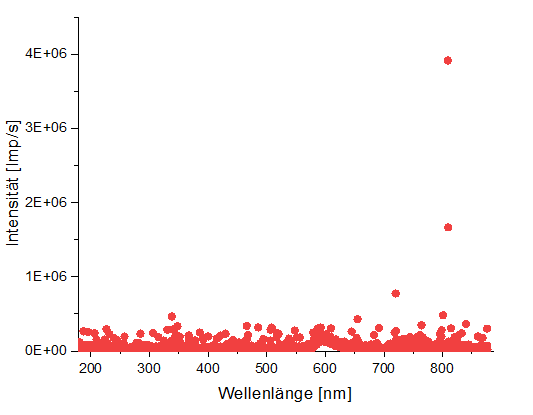
\includegraphics[scale = 1.5]{peak.png}
	\caption{Spektrum der durch den Stickstofflaser gepumpten Farbstoffes im sichtbaren Bereich}
	\label{Farbstoff}
\end{figure}
Somit wird nur noch der kleinere Peak betrachtet. Mit dem emittierten Licht in diesem Bereich kann auf die Zusammensetzung des Farbstoffes geschlossen werden. In \cref{cool} ist dieser Bereich vergrößert dargestellt.
\begin{figure}[h!]
	\centering
	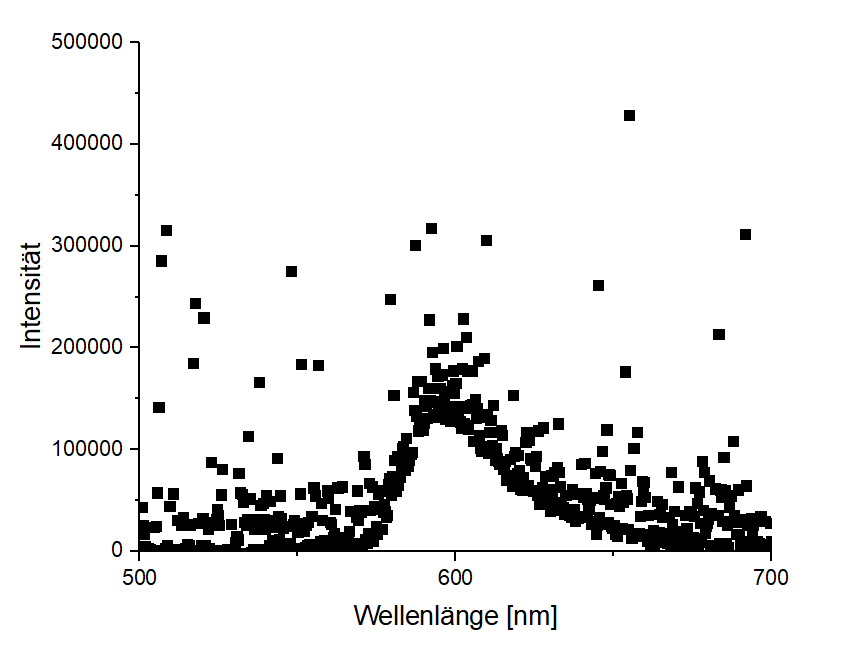
\includegraphics[scale = 1]{cool.png}
	\caption{Dies stellt eine Vergrößerung von \cref{Farbstoff} dar.}
	\label{cool}
\end{figure}
Ein Vergleich mit folgender Tabelle führt uns auf zwei Stoffe.
\begin{figure}[h!]
	\centering
	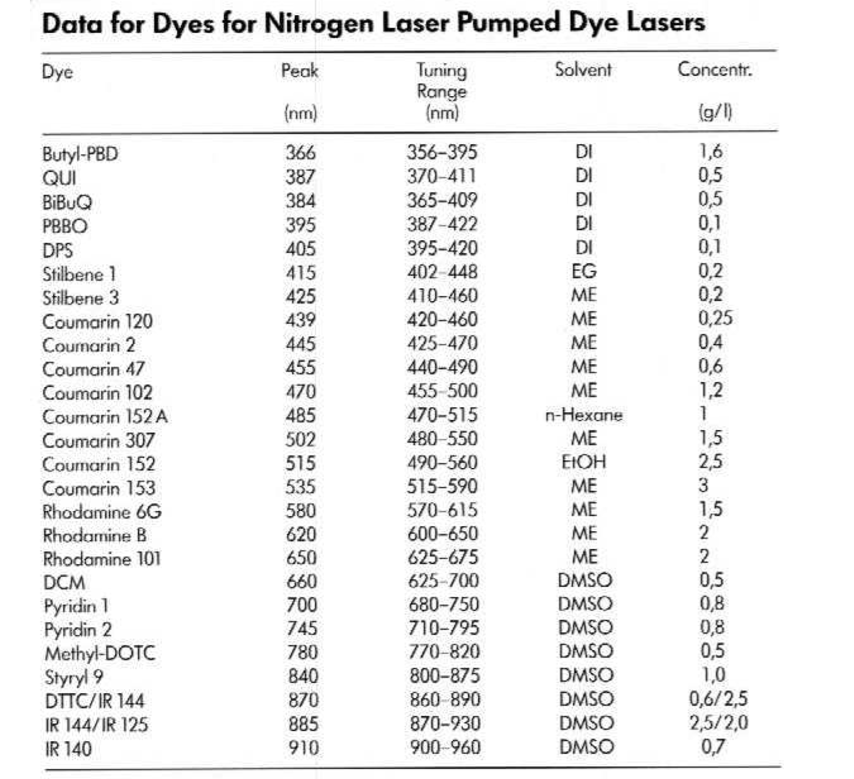
\includegraphics[scale = 1]{data.png}
	\caption{Dies stellt eine Vergrößerung von \cref{Farbstoff} dar.}
	\label{cool}
\end{figure}
Coumarin 153 und Rhodamine 6G könnten beide Stoffe sein. Da der Peak im gesamten Bereich vorhanden ist, ist der Farbstoff ein Gemisch aus beiden Stoffen.

\subsection{Unsicherheiten}
Die theoretische Berechnung der Linienbreite wurde als exakt angenommen, da die einzelnen Komponenten alle einen so geringen Fehler besitzen, dass diese zu der angegebenen Anzahl an Stellen des theoretisch berechneten Ergebnisses vernachlässigbar klein sind.
Hingegen sind die Fehler des experimentellen Versuchs auf 3\% für die Messung der Intensität festgesetzt worden und für die Wellenlängenmessung auf
$0,02$nm. Die Messfehler wurden nur in den Grafiken eingebaut, mit deren Graphen Rechnungen durchgeführt worden sind. Die Unsicherheiten für die Halbwärtsbreite wurden durch das Program OriginPro berechnet. 


\subsection{Diskussion}
In diesem Teil muss man sich mit zwei zentralen Aufgabenstellungen nochmal auseinandersetzen. Der erste Teil bezieht sich auf das aufgenommene Spektrum. 
Innerhalb der Auswertung konnte keine Zuordnung des Nebenpeaks gefunden werden, sodass hier ein Effekt zu beobachten ist, der durch die Theorie nicht beschrieben wurde. 
Der zweite Aspekt der zu diskutiere übrig bleibt, ist die Diskrepanz zwischen Experiment und Theorie. Hier liegt ein Größenunterschied von einem Faktor 1000 dazwischen. Da der Peak in Sättigung betrieben wurde ist, wie bereits oben erklärt, nur eine obere Grenze festzustellen. Dennoch sollte diese Grenze nicht um einen Faktor 1000 daneben liegen, da es bereits eine Korrektur der Messdaten vorgenommen wurde und ein Gaußförmiger Verlauf angenommen wurde. Der verlauf kann als gute Approximation angenommen werden, da diese genau die Wahrscheinlichkeitsverteilungen aus theoretischen Überlegnungen entsprechen. Sodass wir zu dem Schluss kommen, dass auf der theoretsichen Seite etwas schief gelaufen sein musste. Da es sich um einen faktor 1000 handelt, der diese Ergebnisse proportional voneinander trennt ist ein Fehler in den Einheiten zu vermuten.
\end{document}
